
No matter what classification techniques it is used, the images have to be transformed into certain kind of feature vectors with one of the
methodologies mentioned above. Image filter (also called \emph{kernel}) allows you to apply various effects on photos. In a 2D image, the 2D filter matrix \emph{f}
 can be applied with a convolutionary operation on the image \emph{I}:
\begin{equation}\label{eq:conv}
\left( {f * I} \right)\left( {x,y} \right) = \iint {f(x,y)I(x - t,y - t)dt}
\end{equation}

\begin{table}
  \centering
\begin{tabular}{|c| c| c|}
  \hline
  original & $\left[ {\begin{array}{ccc}  0&0&0 \\  0&1&0 \\  0&0&0\end{array}} \right] $ &\parbox[c]{5em}{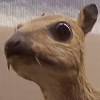
\includegraphics[scale=1.5]{fig/orig.png}}\\
  \hline
  edge detect & $\left[ {\begin{array}{ccc}  -1&-1&-1 \\  -1&8&-1 \\  -1&-1&-1\end{array}} \right] $ & \parbox[c]{5em}{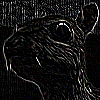
\includegraphics[scale=1.5]{fig/edge.png}}\\
  \hline
  blur & $\left[ {\begin{array}{ccc}  1&1&1 \\  1&1&1 \\  1&1&1 \end{array}} \right] $ & \parbox[c]{5em}{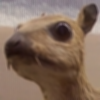
\includegraphics[scale=1.5]{fig/blur.png}}\\
  \hline
\end{tabular}
  \caption{Apply filters on image}\label{kl}
\end{table}

For a image classification task, the key issue is to find the most useful features to present the image. The results of the classification results can be greatly affected by the type of the kernels used. So there are two essential parts here: how to get the kernels and how to present the image with these kernels and the second part of the problem can be considered as the encoding the features. There are 3 different kernels defined in Table \ref{tab:edge}. After applying these kernels on the original image, the results are shown in the 3rd column. The size of the kernel can affect the image: the smaller the kernel is, it is more sensitive to some features in the image. However, the larger one is also useful while there are some noisy in the image as it is less possible to detect those tiny noisy pixels. From Furthermore there are many different kinds of kernels (with different properties and sizes) that can applied on the image to detect different features. For a specific problem, it is very difficult and inefficient to define any kernels even though we may acquire sufficient prior knowledge for this problem. And as the develop of the power of the computer and the complexity of the problem, it is not possible for one to get enough prior knowledge.
 \begin{figure}
  \centering
  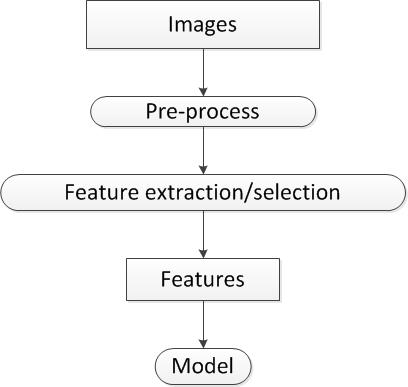
\includegraphics[scale=0.6]{fig/proces.jpg}\\
  \caption{Image Classification Procedure}
\end{figure}


\begin{table}
  \centering
  \begin{tabular}{cccc}
     \hline
     Original & Vertical Kernel 1 & Vertical Kernel 2 & Vertical Kernel 3\\
      \hline
      $\left[ {\begin{array}{ccc}  0&0&0 \\  0&1&0 \\  0&0&0\end{array}} \right] $
      & $\left[ {\begin{array}{ccc}  1&0&-1 \\  5&0&-5 \\  1&0&-1\end{array}} \right] $
      &$\left[ {\begin{array}{ccc}  -1&0&-1 \\  2&0&-2 \\  1&0&-1\end{array}} \right] $
      & $\left[ {\begin{array}{ccccc}   1     & 2     & 0     & -2    & -1 \\    4     & 8     & 0     & -8    & -4 \\    6     & 12    & 0     & -12   & -6 \\    4     & 8     & 0     & -8    & -4 \\    1     & 2     & 0     & -2    & -1 \\ \end{array}} \right]$\\
     \hline
     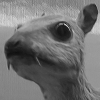
\includegraphics[scale=.5]{fig/gray.png} & 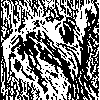
\includegraphics[scale=.5]{fig/v1.png}
     &  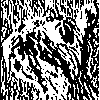
\includegraphics[scale=.5]{fig/v2.png}  &  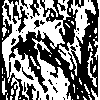
\includegraphics[scale=.5]{fig/v4.png}\\
     \hline
   \end{tabular}
  \caption{Different Kernels for Edge Detection}\label{tab:edge}
\end{table}

For a more heuristic way, many researchers try to learn the specific kernels for a particular task with either supervised or unsupervised learning strategies \cite{Berkes:2005}\cite{SVM99}\cite{hinton06}\cite{LeCun12}\cite{LeRMDCCDN12}. In kernel methods, the problem is modeled as a pairwise relation between data points which is captured in kernels. Thus, kernel functions (or simply kernels) have a profound impact on the performance of these learning algorithms \cite{AbbasnejadRR12}. However, tuning the kernels to fit the underlying hypotheses of the dataset can be a great challenge. As the images are taken in different situations, the light condition, the angle of the view and the shadow of the objects in the image would affect the performance of the kernels. On the other hand, mathematically kernel learning can be a constrained optimization task. Good kernels can map the images into high dimensional space which makes them more distinguishable. In an image recognition task, the image always includes at least thousands of pixels and there are also thousands of images for training. Optimization on these large high dimensional dataset, taking gradient descent for instance, can easily stuck into local minimum no matter how simple the objective function is. Also kernel learning can be considered as a problem similar to distance metric learning as the pixels in the image can be "activated" by a kernel if they are similar. But distance metric learning is trivial in image recognition which would be affected by many simple geometrical transformation such as rotation, shift or zoom in/out. In human brain, we do this unconsciously and parallelling. Many conventional distance metrics have been used in computer vision even though none these metrics can handle geometrical transformation. Thus before measuring the distance of the original image and the kernels, some transformations have to be apply on the original image such as rotation with different degrees (like from -30 degree to 30 degree with 1 degree interval), shift around (within a $9\times9$ window) and scaling in order to fit the kernel. Within these operations, maybe just one set of the combinations can have a high response which we couldn't know in advance. Yann LeCun \emph{et al} introduced \emph{ConvNet} which applies convolutionary operation on the whole image to learning the kernels\cite{Yann98}. Still ConvNet is one of the most popular methods with the best performance in real world image recognition\cite{CiresanIJCAI11}\cite{RanzatoNIPS06}\cite{KrizhevskyNIPS12}.

\begin{flushleft}
\emph{City Block Distance/Manhattan Distance}
\end{flushleft}
\begin{equation}
  d({P_1},{P_2}) = \sum\limits_{i = 1}^n {\left| {p_1^i - p_2^i} \right|}
\end{equation}

\begin{flushleft}
\emph{Euclidean Distance}
\end{flushleft}
\begin{equation}
  d({P_1},{P_2}) = \sqrt {\sum\limits_{i = 1}^n {{{\left( {p_1^i - p_2^i} \right)}^2}} }
\end{equation}

\begin{flushleft}
\emph{Cosine Distance}
\end{flushleft}
\begin{equation}
  d({P_1},{P_2}) = 1 - \frac{{{P_1}{P_2}^T}}{{\left\| {{P_1}} \right\|\times\left\| {{P_2}} \right\|}}
\end{equation}

As each image normally contains thousands of pixels, cutting the image into small patches can be a more realistic way when learning the kernels. 